\subsection{Implementación SRGAN.}

La implementación de este modelo se realizara utilizando la arquitectura presentada
en \cite{SRGAN} mediante el lenguaje \emph{Python} utilizando la librería de alto nivel \emph{Keras}

Keras es una API que proporciona numerosos bloques
de construcción útiles los cuales pueden ser conectados para crear arquitecturas de
aprendizaje profundo altamente complejas.

Para el entrenamiento de las redes, Keras utiliza una de las tres librerías como
\emph{backend} para este propósito: \emph{TensorFlow}, \emph{CNTK}, o \emph{Theano}. Para esta implementación
se utiliza \emph{TensorFlow}, que es una librería de Python de código abierto para el
aprendizaje automático, esta fue desarrollada por Google.


\subsubsection{Modelo generador.}

\begin{figure}[H]
  \begin{center}
    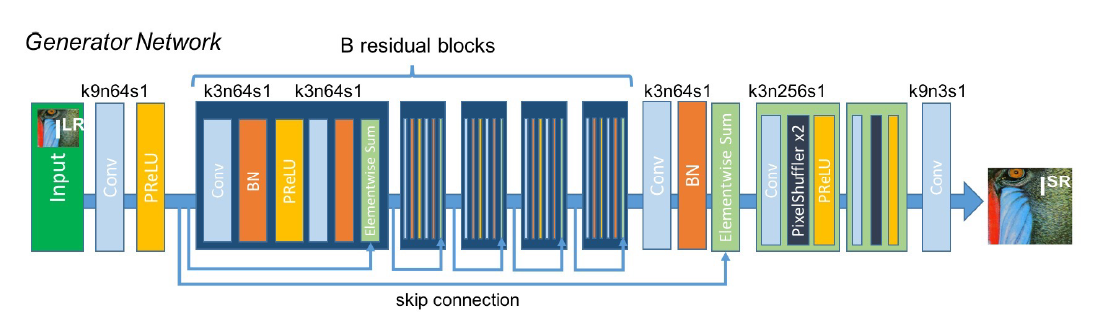
\includegraphics[scale = 0.6]{Imp_generador.png}
    \caption{Arquitectura del generador de la SRGAN,\emph{k} es el tamaño del
    filtro, \emph{n} es la dimensión del mapa de características (capa convolucionada) y \emph{s} indica
    el valor del parámetro stride. Imagen tomada de \cite{SRGAN}}
    \label{Alexis4}
  \end{center}
\end{figure}

\subsubsection{Modelo discriminador.}

\begin{figure}[H]
  \begin{center}
    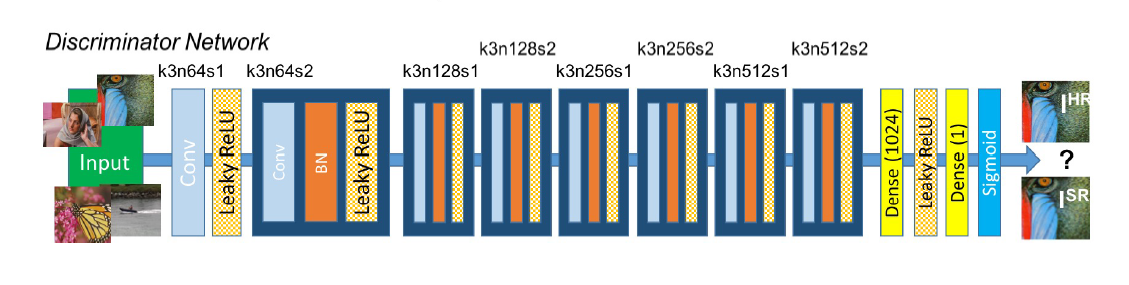
\includegraphics[scale = 0.6]{Imp_discriminador.png}
    \caption{Arquitectura del Discriminador de la SRGAN, \emph{k} es el tamaño
    del filtro, \emph{n} es la dimensión del mapa de características (capa convolucionada) y \emph{s}
    indica el valor del parámetro stride. Imagen tomada de \cite{SRGAN}}
    \label{Alexis5}
  \end{center}
\end{figure}

\subsubsection{Entrenamiento}

EL modelo de entrenamiento de las GAN´s

\begin{figure}[H]
    \begin{center}
      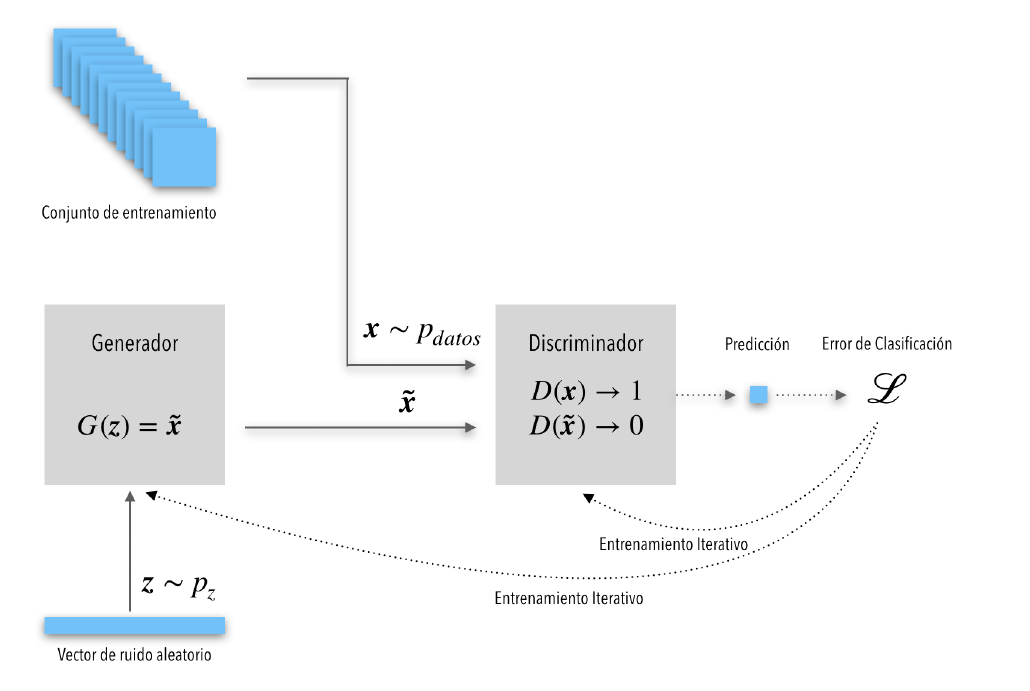
\includegraphics[scale = 0.6]{proceso_gan.png}
      \caption{Proceso de entrenamiento}
      \label{Alexis6}
    \end{center}
\end{figure}